\documentclass[tikz,border=8pt]{standalone}
\usepackage{tikz}
\usetikzlibrary{shapes,arrows,positioning}
\tikzstyle{proc}=[rectangle,draw,rounded corners,fill=blue!10,align=center,minimum width=3.4cm,minimum height=0.9cm,font=\small]
\tikzstyle{dec}=[diamond,draw,fill=green!10,align=center,aspect=2,font=\small]
\tikzstyle{term}=[rectangle,draw,rounded corners=8pt,fill=gray!15,align=center,minimum width=2.6cm,minimum height=0.9cm,font=\small\bfseries]
\tikzstyle{arr}=[->,thick]
\begin{document}
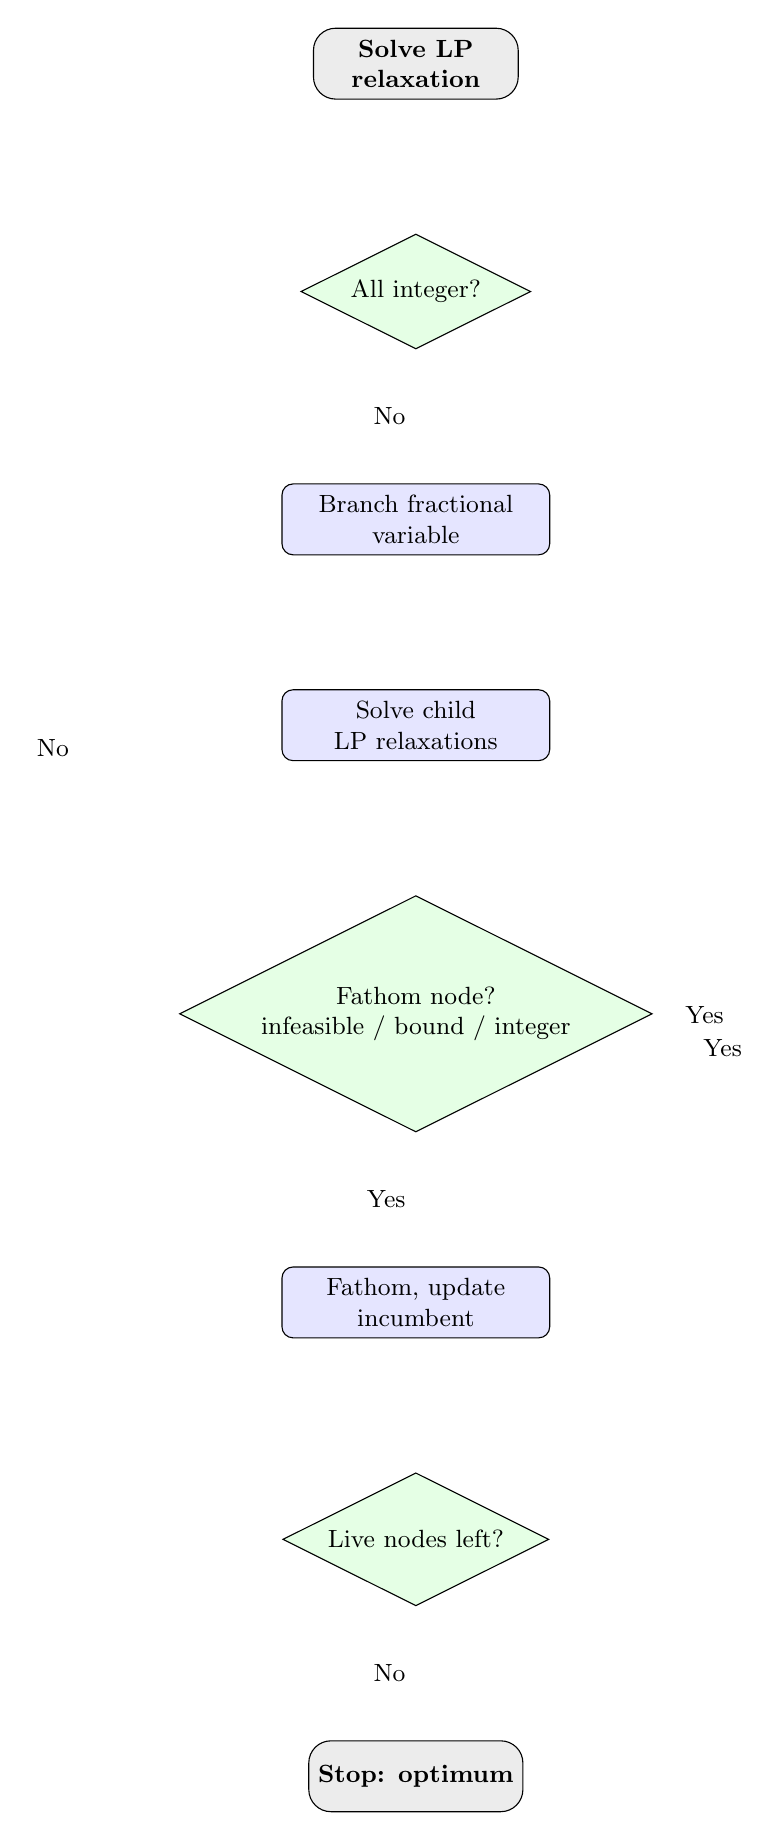
\begin{tikzpicture}[node distance=1.7cm]
\node[term] (A) {Solve LP\\relaxation};
\node[dec, below=of A] (B) {All integer?};
\node[proc, below=of B] (D) {Branch fractional\\variable};
\node[proc, below=of D] (E) {Solve child\\LP relaxations};
\node[dec, below=of E] (F) {Fathom node?\\infeasible / bound / integer};
\node[proc, below=of F] (G) {Fathom, update\\incumbent};
\node[dec, below=of G] (H) {Live nodes left?};
\node[term, below=of H] (C) {Stop: optimum};
\path[arr] (A) -- (B);
\path[arr] (B) -- node[left, font=\small] {No} (D);
\path[arr] (D) -- (E);
\path[arr] (E) -- (F);
\path[arr] (F) -- node[left, font=\small] {Yes} (G);
\path[arr] (G) -- (H);
\path[arr] (H) -- node[left, font=\small] {No} (C);
\path[arr] (B.east) -- ++(2.2cm,0) |- node[near start, above, font=\small] {Yes} (C.east);
\path[arr] (F.west) -- ++(-1.6cm,0) |- node[near start, above, font=\small] {No} (D.west);
\path[arr] (H.east) -- ++(2.2cm,0) |- node[near start, below, font=\small] {Yes} (D.east);
\end{tikzpicture}
\end{document}
